\subsubsection{Exercise}

In this exercise we calculate 4 controllers for the four tank process based on the values of the effective outlet hole areas, the $k_i$ and $\gamma_i$ ($i=1,2$). 

The four controller (two for the minimum phase case and two for non-minimum phase case) are calculated based on the work made during the computer exercise of the course \cite{exo4}. 

The first two controller are decentralized controller. The two other are Glover-MacFarlane controllers.

We want to fulfill the following specifications:
\begin{shortitemize}
    \item Phase margin $\phi_m = \pi/3$,
    \item Cross-over frequency:
        \begin{shortitemize}
            \item $\omega_c = 0.1$ rad/s for the minimum phase case,
            \item $\omega_c = 0.02$ rad/s for the non-minimum phase case.
        \end{shortitemize}
\end{shortitemize}

\paragraph{Decentralized control and decoupling}

Since input and ouptut signals are coupled we try to make a better system using \emph{decoupling}. 
Two solutions can be used: static decoupling and dynamical decoupling. 
Static decoupling is obtained by decoupling the system at a given frequency.
Dynamical decoupling take care of decoupling the system for each frequency.
According to the results obtain in the computer exercises we chose the dynamical decoupling. (better results regarding the sentivity and robustness). 
We obtained the decoupled system with the method depicted in \cite{exo4}.
We used decoupled PI-controller. The following table sum up our results:

\begin{center}
\begin{tabular}{|c|cccc|}
    \hline
    \multicolumn{5}{|c|}{PI controllers} \\
    \hline
    & $K_1$ & $K_2$ & $T_1$(s) & $T_1$(s) \\ 
    Minimum case & $1.63$ & $1.96$ & $5.80$ & $6.28$\\
    Non-minimum case &  $1.13$ & $0.94$ & $22.40$ & $23.44$ \\
    \hline
\end{tabular}
\end{center}

Figure \ref{sensfunction} shows the sensitivity and complementary sensitivity function for each case using the PI decentralized controllers.

\begin{figure}[h!t]
        \centering
        \begin{subfigure}[b]{0.45\columnwidth}
                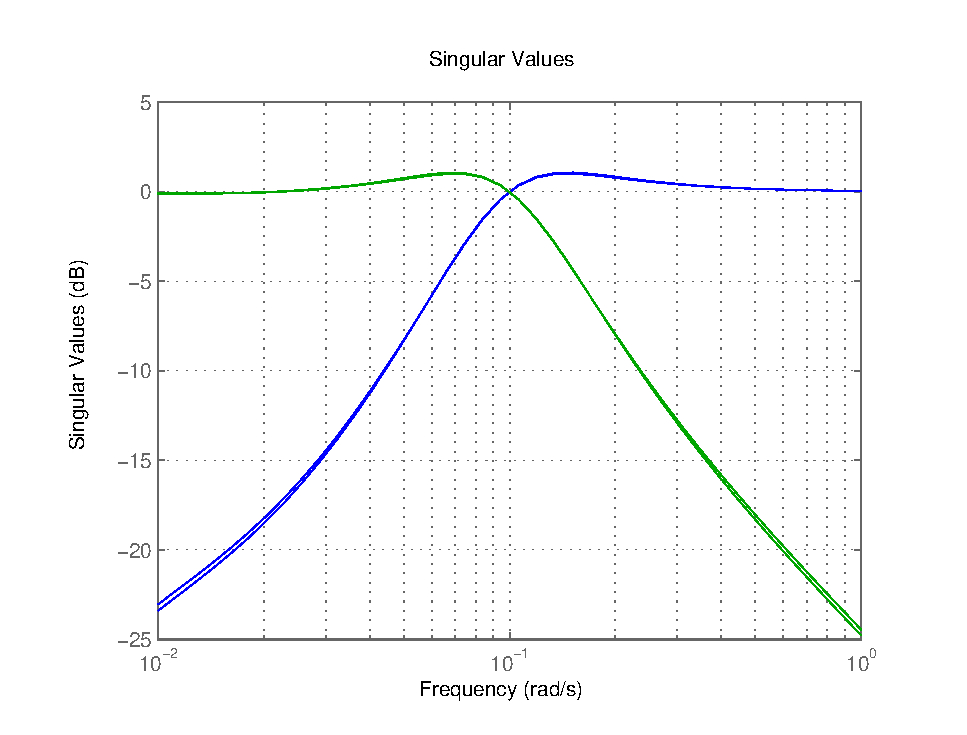
\includegraphics[width=\columnwidth]{fig/sensitivity_dyn_minphase.eps}
                \caption{Minimum phase case}
        \end{subfigure}
        \begin{subfigure}[b]{0.45\columnwidth}
                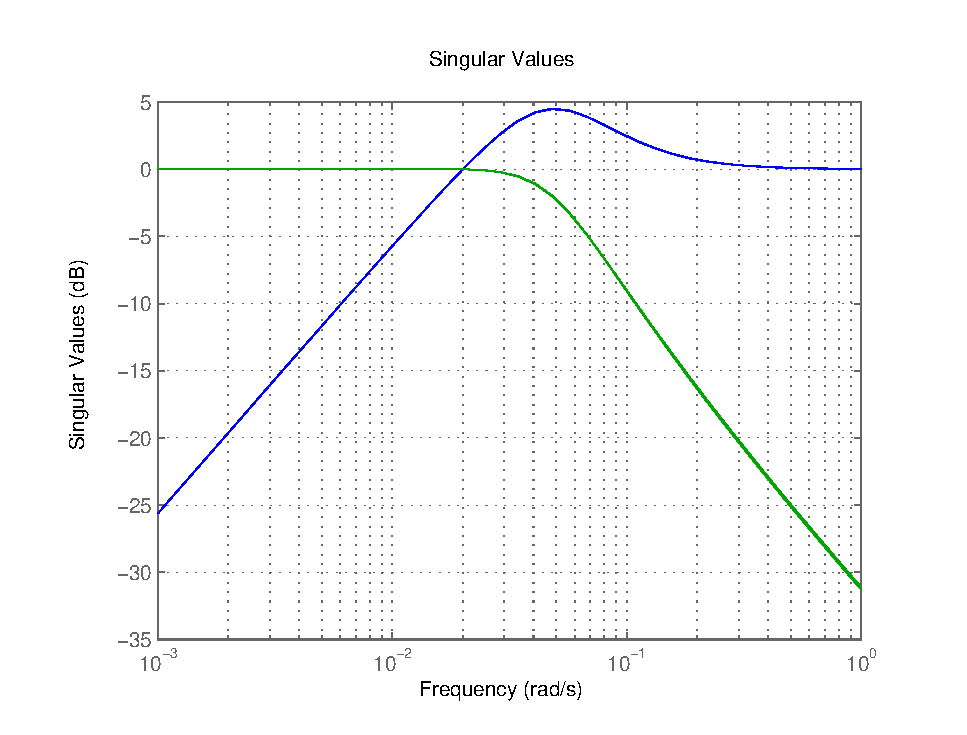
\includegraphics[width=\columnwidth]{fig/sensitivity_dyn_nonminphase.eps}
                \caption{Non-minimum phase case}
        \end{subfigure}
        \caption{Sensitivity and complementarity function using PI decentralized controllers}
        \label{sensfunction}
\end{figure}


\paragraph{Glover-MacFarlane controller}

The decentralized control obtained in the previous paragraph is then robustified using the Glover-MacFarlane method (using once again the method depicted in \cite{exo4}). 

Figure \ref{sensfunctionglover} shows the sensitivity and complementary sensitivity function for each case using the robustified controller.

\begin{figure}[h!t]
        \centering
        \begin{subfigure}[b]{0.45\columnwidth}
                \includegraphics[width=\columnwidth]{fig/sensitivity_glover_minphase.eps}
                \caption{Minimum phase case}
        \end{subfigure}
        \begin{subfigure}[b]{0.45\columnwidth}
                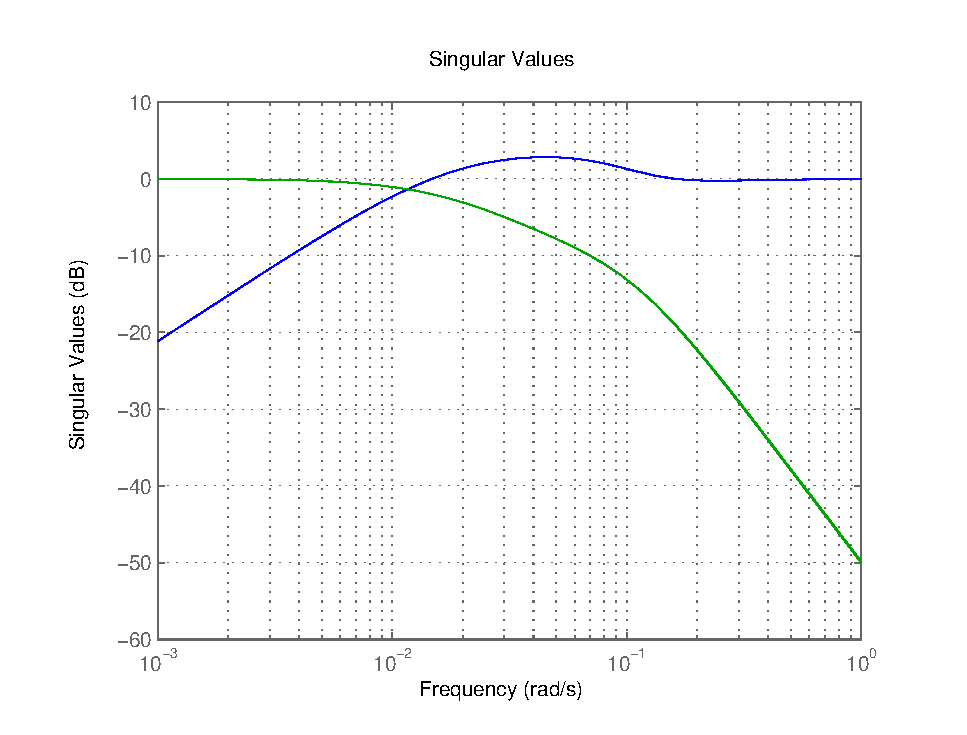
\includegraphics[width=\columnwidth]{fig/sensitivity_glover_nonminphase.eps}
                \caption{Non-minimum phase case}
        \end{subfigure}
        \caption{Sensitivity and complementarity function using Glover-MacFarlane controller}
        \label{sensfunctionglover}
\end{figure}

As we can see with Figures \ref{sensfunction} and \ref{sensfunctionglover} the system seems more robust using the Glover-MacFarlane controllers (maximum gain of $S$ and $T$ and bandwiths are smaller).
